% \documentclass[german,bachelor,ul]{webisthesis} % Weimar
% \documentclass[german,bachelor,fsu]{webisthesis} % Jena
\documentclass[english,bachelor,ul]{webisthesis} % Leipzig
%
% Non-default programme
% ---------------------
% \documentclass[english,master,buw]{webisthesis}\global\thesisprogramme{Human-Computer Interaction}
% \documentclass[english,master,buw]{webisthesis}\global\thesisfrontpagefaculty{Faculty of Civil Engineering/Faculty of Media}\global\thesisprogramme{Digital Engineering}
% \documentclass[german,bachelor,buw]{webisthesis}\global\thesisprogramme{Informatik\\Schwerpunkt Medieninformatik}
% \documentclass[german,bachelor,buw]{webisthesis}\global\thesisprogramme{Informatik\\Schwerpunkt Security and Data Science}
%
% When you change the language, pdflatex may halt on recompilation.
% Just hit enter to continue and recompile again. This should fix it.


%
% Values
% ------
\ThesisSetTitle{The Title of the Thesis}
\ThesisSetKeywords{These, are, my, Keywords} % only for PDF meta attributes
\ThesisSetLocation{Leipzig} 

\ThesisSetAuthor{Yannick Brenning}
\ThesisSetStudentNumber{3732848}
\ThesisSetDateOfBirth{27}{8}{2002}
\ThesisSetPlaceOfBirth{Bamberg}

% Supervisors should usually be Professors from the candidate's university. A second supervisor is not always needed. 
\ThesisSetSupervisors{Christopher Schröder, Christian Kahmann}

\ThesisSetSubmissionDate{31}{2}{2022}

%
% Suggested Packages
% ------------------
\usepackage[sort&compress]{natbib}
%   Allows citing in different ways (e.g., only the authors if you use the
%   citation again within a short time).
%
\usepackage{booktabs}
%    For tables ``looking the right way''.
%
% \usepackage{tabularx}
%    Enables tables with columns that automatically fill the page width.
%
% \usepackage[ruled,algochapter]{algorithm2e}
%    A package for pseudo code algorithms.
%
% \usepackage{amsmath}
%    For tabular-style formatting of mathematical environments.
%

\usepackage{fontawesome}
%    For lots of awesome glyphs: https://mirror.physik.tu-berlin.de/pub/CTAN/fonts/fontawesome/doc/fontawesome.pdf

\usepackage{multirow}
\usepackage{pdfpages}
\usepackage{graphicx}

%
% Commenting (by your supervisor)
% -------------------------------
\usepackage{xcolor}
\usepackage{soul}
\newcommand{\bscom}[2]{%
  % #1 Original text.
  % #2 Replacement text.
    \st{\scriptsize\,#1}{\color{blue}\scriptsize\,#2}%
  }

% Create links in the pdf document
% Hyperref has some incompatibilities with other packages
% Some other packages must be loaded before, some after hyperref
% Additional options to the hyperref package can be provided in the braces [], like in
% \usehyperref[backref] % This will add back references in the bibliography that some people like ... some don't ... so better ask your supervisor ;-)
\usehyperref

\begin{document}
\begin{frontmatter}
\begin{abstract}
This is the \LaTeX{} template for Bachelor and Master theses at Webis. This template contains several hints and conventions on how to structure a thesis, how to cite the work of others, and how to display your results besides plain text. 
\end{abstract}
\end{frontmatter}

\tableofcontents

\chapter{Introduction}

Text is one of the most widespread and important sources of information, but extracting data and tangible knowledge from it can be a difficult and expensive task. With the advent of the digital age, enormous amounts of unstructured texts are available with more being generated by the day. Due to this increasingly large amount of textual data, processing information at a larger scale becomes infeasible and thus demands the use of computer-driven approaches. 

The classification of text, meaning the assignment of a category or class to a document or piece of text is one of the most common and useful ways to gain information from a piece of text. As the amount of available text content continues to grow, text classification tasks become an increasingly important area of research within the field of natural language processing. 

Thanks to machine learning and data science, we have been able to develop many methods of extracting information from text, and as a result, perform text classification at a larger scale. This possibility for automated organization of data can enhance insights and decision-making across industries such as healthcare, finance, and social sciences, among many others. Active Learning (AL) is a subfield of machine learning in which the learning algorithm is able to perform queries on an information source in order to reduce the total amount of annotated data. This method can offer significant advantages in improving model performances and especially in reducing labeling costs. Though there is no universally good strategy, AL has been proven to be useful in many cases where annotating data is expensive or the total amount of data is very large (\cite{settles.tr09}). 

% One such model is the CNN (convolutional neural network), which is used in many recognition and learning tasks but needs to be trained on a large dataset. With AL, selecting the most effective data points to be labelled by the oracle from a large pool of unlabelled data can be a challenge, especially in the case of CNNs. 
Oftentimes, there is a large amount of unlabelled available data for an AL model to learn from. In this case, selecting the most effective data points to be labelled by the information source from this large pool becomes a crucial, but difficult challenge to overcome. 

One attempt at improving the effectiveness of AL in this regard is the Core-Set approach (\cite{DBLP:conf/iclr/SenerS18}) This method uses core-set selection to counter the issue of AL ineffectiveness on convolutional neural networks. The proposed approach selects a set of points the pool such that a model learning over this subset can be consistent when provided the remaining data points. The method was shown to have improved results when compared to other approaches in the field of computer vision (\cite{DBLP:conf/iclr/SenerS18}, \cite{DBLP:conf/cvpr/CaramalauBK21}), which encompasses tasks that focus on enabling computers to interpret and understand visual information from the world. This field involves a variety of different methods including image classification, object detection, and semantic segmentation, all of which have significant importance in scientific research, classification tasks, and pattern recognition.

However, Core-Set has been shown to have mixed results in cases of multi-class text classification using BERT (\cite{DBLP:conf/kdd/0002MM21}) and binary text classification using DNNs (\cite{DBLP:conf/cikm/Liu0LZW21}). Particularly in the first case, the experiments show that Core-Set performs poorly even when compared to the random sampling strategy. In addition, the approach has even been shown to be less effective in computer vision tasks in cases with higher numbers of classes as well as higher-dimensional data points (\cite{DBLP:conf/iccv/SinhaED19}). The theoretical analysis shown in \cite{DBLP:conf/iclr/SenerS18} briefly mentions this within the context of higher class amounts, however it does not attempt to provide a potential solution to the problem.

% Particularly in first case, the experiments conducted on the Internal Dataset and TREC-6 show that Core-Set performs poorly when comparing the F1-scores to the random sampling strategy. 

This thesis aims to explore the possibility of improving the Core-Set approach for text classification tasks. By first explaining Core-Set's functionality and the theoretical reasons for why it tends to underperform in certain classification tasks, I aim to then demonstrate the performance difference in comparison to various baseline approaches on large datasets of text content in order to verify this claim. Furthermore, this thesis looks to improve on the Core-Set approach within the context of text classification tasks and demonstrate this improvement as a part of its experiment.

In the following, Chapter 2 explains the background and related work on the topics of text classification (Section 2.1), active learning in general (Section 2.2), and the Core-Set approach to AL more specifically (Section 2.3). In Chapter 3, I will explain my approach to improving the performance of Core-Set for text classification using dimensionality reduction. In Chapters 4 and 5, I will present my experiment as well as discuss its results. Finally, Chapter 6 will conclude the thesis and provide insights on potential future developments of the method. 

\chapter{Background/Related Work}

\section{Text Classification}

% **GENERAL**
Text classification is one of the most fundamental and important tasks in the field of Natural Language Processing (NLP). As a result, developing efficient automatic text classification methods has become an important research topic. 

% **APPLICATION**
One of the most common applications of text classification is determining whether the opinion associated with a certain document has a positive or negative sentiment, also known as sentiment analysis. This has a wide range of uses, including the possibility for businesses to better gauge customer opinions on products and services (\cite{DBLP:books/sp/mining2012/LiuZ12}) in order to adapt accordingly. This application is a binary classification task, meaning the classifier has two classes with which each document can be labelled (positive or negative). Similarly, one might apply this binary classification task to the problem of spam filtering in e-mails, text messages and more. 

Beyond that, many applications of text classification require multiple classes, such as news and content categorization. In this case, text classification algorithms can organize documents into specific topics or themes (e.g. Sports, Business, Politics, \dots) (\cite{DBLP:journals/csur/Sebastiani02}). Other applications include information retrieval, recommender systems, and document summarization (\cite{DBLP:journals/information/KowsariMHMBB19}).

% **PROCESS**
Generally, text classification methods can be divided into the following phases: data collection and preprocessing, feature extraction, classifier selection, and model evaluation (\cite{DBLP:journals/information/KowsariMHMBB19}, \cite{DBLP:journals/eswa/MironczukP18}, \cite{ikonomakis2005text}).

% **CHALLENGES(?)**

\section{Active Learning}

\section{Core-Set}

\section{Dimensionality Reduction}

As mentioned earlier, one of the major challenges of the Core-Set approach (among others) is handling data points with a higher dimensionality (\cite{DBLP:conf/iccv/SinhaED19}). Broadly speaking, this is a phenomenon coined by Richard E. Bellman known as the \textit{curse of dimensionality} (\cite{franccois2007high}). As a result, many algorithms have been developed to transform data from a high-dimensional space into a low-dimensional space. This task directly poses another challenge: managing to reduce the dimensionality of the data while still being able to retain the highest possible amount of information. 

One such method is the Principal Components Analysis (PCA), which is one of the most popular linear techniques for dimensionality reduction (\cite{van2009dimensionality}). In essence, PCA linearly transforms the data into a representation that attempts to closely describe the variance of the initial data (\cite{jolliffe2016principal}). Other commonly used linear techniques include Linear Discriminant Analysis (LDA), Multidimensional Scaling (MDS), and Non-negative Matrix Factorization (NMF).

These techniques can be powerful, however they often miss important non-linear structures in high-dimensional data. Therefore, non-linear techniques have been developed such as Isometric Mapping (Isomap) and t-distributed Stochastic Neighbor Embedding (t-SNE). The latter is a relatively modern probablistic approach that has improved upon many other non-linear techniques in creating a single map that reveals structure on many different scales. In addition, it manages to reduce the tendency of SNE to crowd data points together at the center by using a different cost function (\cite{van2008visualizing}). 

First, it converts the high-dimensional Euclidean distances into conditional probabilities, such that similar data points are assigned higher probabilities and dissimilar data points are assigned very low probabilities. It then creates a similar probability distribution over the lower-dimensional map such that the \textit{Kullback-Leibler divergence} (a measure of how one probability distribution differs from another) is minimized.

This method is especially useful for the visualization of high-dimensional data, in which the aim is to display and view the underlying structure in a given dataset. t-SNE plots are strongly influenced by the chosen hyperparameters however, and thus a good understanding for the influence of these parameters is important. Particularly \textit{perplexity}, a measure of the effective number of neighbours, has a complex effect on the resulting reductions. According to \cite{van2008visualizing}, typical values for perplexity are between 5 and 50 and larger/denser datasets often generally require higher perplexities (\cite{vanHomepage}). Other commonly adjusted parameters include the learning rate and number of iterations for the optimization.

\chapter{Approach}

As mentioned, distance-based methods such as Core-Set can be ineffective in higher dimensions. To overcome this challenge, I propose the application of t-SNE as a dimensionality reduction technique on the training data before employing the Greedy Core-Set strategy. In order to optimize my use of t-SNE, I will first examine the effects of different hyperparameters on the reductions. Based on these examinations, I will select the optimal t-SNE parameters to use for the experiment.

As mentioned earlier, setting t-SNE's hyperparameters and exploring the resulting differing reduction behaviours has been shown to often be necessary (\cite{wattenberg2016how}). \cite{vanHomepage} mentions that examining the resulting plots is one of the best ways to assess the quality of the visualizations, in addition to comparing the Kullback-Leibler divergences. 

Below, I have demonstrated the effect of t-SNE on a training set of the well-known Movie Review dataset (\cite{DBLP:conf/acl/PangL05}) containing 9,596 samples with a feature dimension of 768. The reductions are completed using perplexity values of 5, 30, 50 and 100 with iteration counts of 1,000 and 5,000 respectively. 

\begin{figure}[htpb]
    \centering
    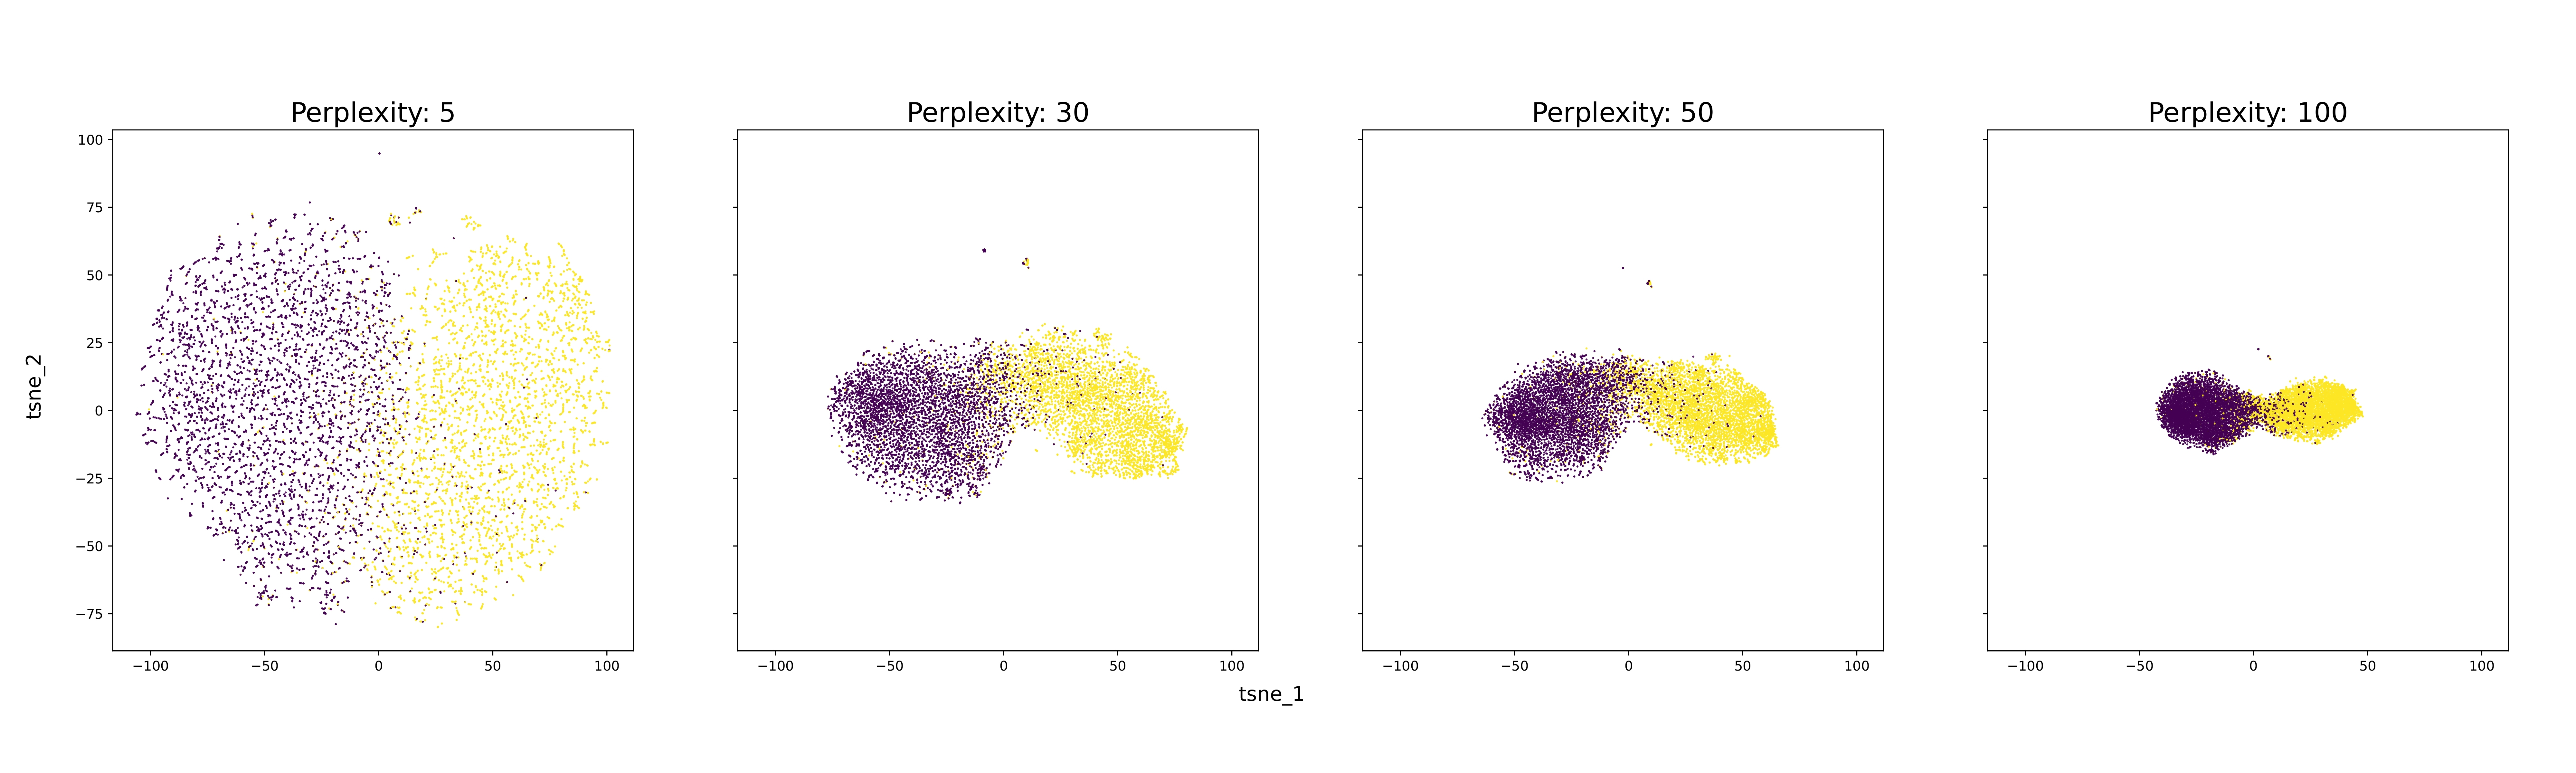
\includegraphics[width=1\textwidth]{reductions-mr-1000.jpg}
    \caption{t-SNE reductions with various perplexity values after 1,000 iterations performed on the embedded and normalized Movie Review dataset.}
    \label{fig:reductions-mr-1000}
\end{figure}

\begin{figure}[htpb]
    \centering
    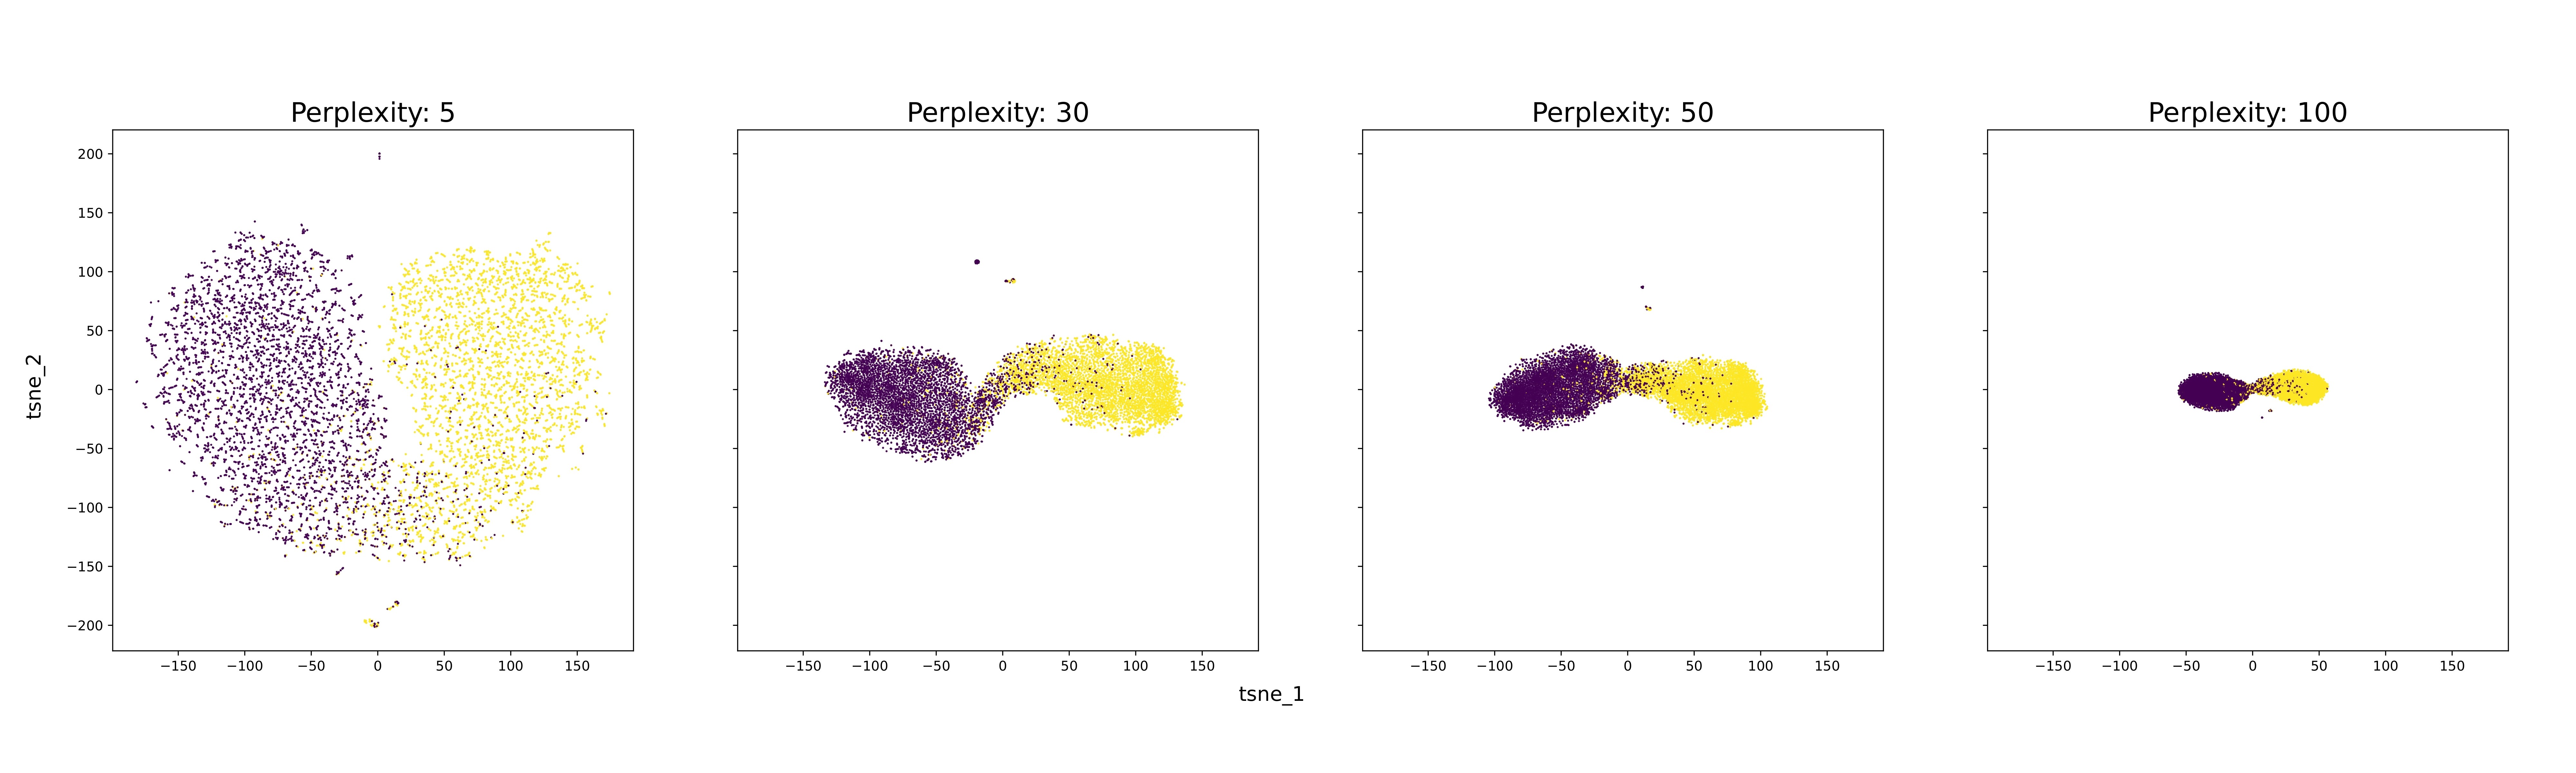
\includegraphics[width=1\textwidth]{reductions-mr-5000.jpg}
    \caption{t-SNE reductions with various perplexity values after 5,000 iterations performed on the embedded and normalized Movie Review dataset.}
    \label{fig:reductions-mr-5000}
\end{figure}

Note that the samples have been embedded using BERT and normalized prior to the dimensionality reductions. \\

Starting at a perplexity of 30, the points begin to cluster more and more tightly. The clusters do not seem to separate in any of the runs -- it is important to note, however, that distances and sizes of the clusters do necessarily carry any meaning when examining the plots (\cite{wattenberg2016how}, \cite{vanHomepage}).

It is also worth noting that the differences between 1,000 and 5,000 iterations appear quite small despite the relative increase in computations.

\chapter{Experiment}

\section{Data}

This experiment was conducted across three datasets commonly used in the field of AL. These datasets are of three different types: sentiment analysis (S), questions (Q), and news (N). For binary classification, I used \textbf{Movie Review}, a sentiment analysis dataset (\cite{DBLP:conf/acl/PangL05}) containing 5,331 positive and 5,331 negative samples. For multi-class text classification, \textbf{AG's News} (\cite{DBLP:conf/nips/ZhangZL15}), comprised of 120,000 training samples and 7,600 test samples, and \textbf{TREC} (\cite{DBLP:journals/nle/LiR06}), a question dataset containing 5,500 training samples and 500 test samples.

The test set was only provided in the case of AG's News and TREC, in the case of Movie Review I employed a split of the 10,662 samples myself. 

% The chosen datasets are Movie Review (MR), a sentiment analysis dataset with 10662 data points, TREC-6, a question dataset with {} data points, and finally AG-News, a topic dataset with 120,000 data points. Each of these datasets is commonly used in the field of AL. One must note that these are comparatively few data points, due to the fact that AL is a time and resource-expensive field.

\section{Experiment Setup}


\section{Experiment Results}

\iffalse
%% TEMPLATE TABLE
\begin{table*}[!t]%
\centering
\fontsize{8pt}{9pt}\selectfont%
\renewcommand{\tabcolsep}{12pt}%
\begin{tabular}{@{}ll@{\hspace{10pt}} r @{${}\pm{}$} r r @{${}\pm{}$} r r @{${}\pm{}$} r r @{${}\pm{}$} r @{}}
\toprule
\textbf{Dataset} & \textbf{Model} & \multicolumn{8}{c}{\textbf{Query Strategy}}\\
\cmidrule{3-10} & & \multicolumn{2}{c}{\hspace*{-6pt}RS} & \multicolumn{2}{c}{BT} & \multicolumn{2}{c}{CS} & \multicolumn{2}{c}{\hspace*{4pt}Unknown}\\
\midrule
\multirow{2}{*}{AGN}  & BERT & 1.852 & 0.415 & 0.907 & 0.203 & \bfseries 0.432 & \bfseries 0.097 & 516.554 & 115.583 \\
 & SetFit & 7.264 & 1.626 & \bfseries 6.199 & \bfseries 1.389 & 10.256 & 2.359 & 481.758 & 142.013 \\
\midrule
\multirow{2}{*}{MR}  & BERT & 0.014 & 0.003 & 0.014 & 0.003 & \bfseries 0.009 & \bfseries 0.002 & 1.889 & 0.425\\
 & SetFit & 0.521 & 0.117 & \bfseries 0.436 & \bfseries 0.098 & 0.468 & 0.105 & 3.672 & 1.098 \\
\midrule
\multirow{2}{*}{TREC-6}  & BERT & 0.085 & 0.019 & 0.042 & 0.009 & \bfseries 0.018 & \bfseries 0.004 & 0.609 & 0.138 \\
 & SetFit & 0.289 & 0.065 & \bfseries 0.248 & \bfseries 0.055 & 1.111 & 0.745 & 1.504 & 0.447 \\
\bottomrule
\end{tabular}
\caption{%
Final accuracy per dataset, model, and query strategy. We report the mean and standard deviation over five runs. The best result per dataset is printed in bold.}
\label{table-results-acc}
\end{table*}
\fi

% MY ACC TABLE
\begin{table*}[!t]%
\centering
\fontsize{8pt}{9pt}\selectfont%
\renewcommand{\tabcolsep}{12pt}%
\begin{tabular}{@{}ll@{\hspace{10pt}} r @{${}\pm{}$} r r @{${}\pm{}$} r r @{${}\pm{}$} r r @{${}\pm{}$} r @{}}
\toprule
\textbf{Dataset} & \textbf{Model} & \multicolumn{8}{c}{\textbf{Query Strategy}}\\
\cmidrule{3-10} & & \multicolumn{2}{c}{\hspace*{-6pt}RS} & \multicolumn{2}{c}{BT} & \multicolumn{2}{c}{CS} & \multicolumn{2}{c}{\hspace*{4pt}CS-TSNE}\\
\midrule

\multirow{2}{*}{AGN}  & BERT & 0.78 & 0.171 & \bfseries 0.79 & \bfseries 0.161 & 0.727 & 0.175 & 0.782 & 0.166\\ 
 & SetFit & 0.862 & 0.044 & \bfseries 0.877 & \bfseries 0.048 & 0.868 & 0.052 & 0.871 & 0.047 \\

\midrule

\multirow{2}{*}{MR}  & BERT & 0.747 & 0.089 & 0.743 & 0.091 & 0.715 & 0.097 & \bfseries 0.749 & \bfseries 0.085\\ 
 & SetFit & 0.853 & 0.015 & \bfseries 0.863 & \bfseries 0.019 & 0.856 & 0.018 & 0.861 & 0.016 \\

\midrule

\multirow{2}{*}{TREC}  & BERT & 0.668 & 0.251 & \bfseries 0.702 & \bfseries 0.246 & 0.592 & 0.256 & 0.671 & 0.251\\ 
 & SetFit & 0.907 & 0.076 & \bfseries 0.916 & \bfseries 0.093 & 0.89 & 0.111 & 0.913 & 0.087 \\
 
\bottomrule
\end{tabular}
\caption{%
Final accuracy per dataset, model, and query strategy. We report the mean and standard deviation over five runs. The best result per dataset is printed in bold.}
\label{table-results-acc}
\end{table*}


% MY AUC TABLE
\begin{table*}[!t]%
\centering
\fontsize{8pt}{9pt}\selectfont%
\renewcommand{\tabcolsep}{12pt}%
\begin{tabular}{@{}ll@{\hspace{10pt}} r @{${}\pm{}$} r r @{${}\pm{}$} r r @{${}\pm{}$} r r @{${}\pm{}$} r @{}}
\toprule
\textbf{Dataset} & \textbf{Model} & \multicolumn{8}{c}{\textbf{Query Strategy}}\\
\cmidrule{3-10} & & \multicolumn{2}{c}{\hspace*{-6pt}RS} & \multicolumn{2}{c}{BT} & \multicolumn{2}{c}{CS} & \multicolumn{2}{c}{\hspace*{4pt}CS-TSNE}\\
\midrule

\multirow{2}{*}{AGN}  & BERT & 0.79 & 0.015 & \bfseries 0.8 & \bfseries 0.009 & 0.735 & 0.02 & 0.792 & 0.007\\ 
 & SetFit & 0.865 & 0.007 & \bfseries 0.881 & \bfseries 0.004 & 0.871 & 0.005 & 0.875 & 0.004 \\

\midrule

\multirow{2}{*}{MR}  & BERT & 0.75 & 0.007 & 0.746 & 0.011 & 0.718 & 0.009 & \bfseries 0.752 & \bfseries 0.016\\ 
 & SetFit & 0.854 & 0.002 & \bfseries 0.864 & \bfseries 0.005 & 0.856 & 0.003 & 0.862 & 0.003 \\

\midrule

\multirow{2}{*}{TREC}  & BERT & 0.674 & 0.029 & \bfseries 0.709 & \bfseries 0.008 & 0.594 & 0.022 & 0.676 & 0.037\\ 
 & SetFit & 0.914 & 0.011 & \bfseries 0.923 & \bfseries 0.007 & 0.896 & 0.015 & 0.919 & 0.005 \\
 
\bottomrule
\end{tabular}
\caption{Final AUC per dataset, model, and query strategy. We report the mean and standard deviation over five runs. The best result per dataset is printed in bold.}
\label{table-results-acc}
\end{table*}

\chapter{Discussion}

\chapter{Conclusion}

% \chapter*{Acknowledgements} % optional
% I thank the authors of the webisthesis template for their excellent work!

% \listoffigures % optional, usually not needed

% \listoftables % optional, usually not needed

% \listofalgorithms % optional, usually not needed
%    requires package algorithm2e

% optional: list of symbols/notation (e.g., using the nomencl package) but usually not needed

%\include{chapter1}
%\include{chapter2}

%\include{appendixA}

% Bibliography
\bibliographystyle{plainnat} % requires package natbib. An alternative is apalike
\bibliography{literature}    % load file literature.bib

\end{document}
